{{ % Localize command definitions

\chapter{Class 7}

For this chapter, we replace the word \emph{formula} in rules and 
proofs of a formal system by the word \emph{judgement}.

\section{Natural Deduction for Propositional Logic}

Judgements in Natural Deduction have the form $\Gamma \vdash \phi$, 
where $\Gamma$ is a set of formulas and $\varphi$ is a formula.
Semantically, for all interpretations $v$, if all formulas in 
$\Gamma$ are true in $v$, then $\phi$ is true in $v$.
Formal system for natural deduction defines a meta-symbol 
$\vdash_\text{meta}$ such that  $\vdash_\text{meta} (\Gamma \vdash 
\phi)$. 

\subsection{Judgements in Natural Deduction}

We use the notation $\Gamma, \phi$ to show $\Gamma \cup \{\phi\}$. 

\begin{enumerate}
  \item Axioms
  \[ \infer* [right=ax]
    { }{\Gamma, \phi \vdash \phi}
    \qquad\qquad \infer* [right=$\top$-intro]
    { }{\Gamma \vdash \top}
  \]
  
  \item False-elimination: if $\bot$ can be derived, then anything 
  can be derived.
  \[ \infer* [right=$\bot$-elim]
    {\Gamma \vdash \bot}{\Gamma \vdash \phi}
  \]

  \item And-elimination and -introduction
  \[ \infer* [right=$\land$-elim]
    {\Gamma \vdash \phi \land \psi}{\Gamma \vdash \phi}
    \qquad\qquad \infer* [right=$\land$-elim]
    {\Gamma \vdash \phi \land \psi}{\Gamma \vdash \psi}
    \qquad\qquad \infer* [right=$\land$-intro]
    {\Gamma \vdash \phi \\ \Gamma \vdash \psi}
    {\Gamma \vdash \phi \land \psi}
  \]

  \item Or-elimination and -introduction
  \[ \infer* [right=$\lor$-elim]
    {\Gamma \vdash \phi \lor \psi 
    \\ \Gamma, \phi \vdash \chi
    \\ \Gamma, \psi \vdash \chi}{\Gamma \vdash \chi}
    \qquad\qquad \infer* [right=$\lor$-intro]
    {\Gamma \vdash \phi}{\Gamma \vdash \phi \land \psi}
    \qquad \infer* [right=$\land$-intro]
    {\Gamma \vdash \phi}{\Gamma \vdash \psi \land \phi}
  \]

  \item Negation-elimination and -introduction
  \[ \infer* [right=$\neg$-elim]
    {\Gamma \vdash \phi \\ \Gamma \vdash \neg \phi}
    {\Gamma \vdash \bot}
    \qquad\qquad \infer* [right=$\neg$-intro]
    {\Gamma, \phi \vdash \bot}{\Gamma \vdash \neg \phi}
  \]
  \item Implication-elimination and -introduction
  \[ \infer* [right=$\rightarrow$-elim]
    {\Gamma \vdash \phi \\ \Gamma \vdash \phi \rightarrow \psi}
    {\Gamma \vdash \psi}
    \qquad\qquad \infer* [right=$\rightarrow$-intro]
    {\Gamma, \phi \vdash \psi}{\Gamma \vdash \phi \rightarrow \psi}
  \]
  Observe how $\rightarrow$-elim is similar to modus ponens.
\end{enumerate}

\begin{homework}
  Prove implication transitivity using Natural Deduction.
\end{homework}

\begin{example}\label{lecture_7:contrapositive}
  Show $(\phi \rightarrow \psi) \rightarrow 
  (\neg \psi \rightarrow \neg \phi)$.
\end{example}
\begin{proof}
  \[ \infer* [right=$\rightarrow$-intro]
    { \infer* [right=$\rightarrow$-intro]
      { \infer* [right=$\neg$-intro]
        { \infer* [right=$\neg$-elim]
          { \phi \rightarrow \psi, \neg \psi, \phi \vdash \psi \\
            \phi \rightarrow \psi, \neg \psi, \phi \vdash \neg \psi
          }{\phi \rightarrow \psi, \neg \psi, \phi \vdash \bot}
        }{\phi \rightarrow \psi, \neg \psi \vdash \neg \phi}
      }{(\phi \rightarrow \psi) 
        \vdash (\neg \psi \rightarrow \neg \phi)}
    }{\vdash (\phi \rightarrow \psi) 
      \rightarrow (\neg \psi \rightarrow \neg \phi)}
  \]
  Now we have two goals to prove. 
  \[ \infer* [right=$\rightarrow$-elim]
    { \infer* [right=ax]
      { }{\phi \rightarrow \psi, \neg \psi, \phi \vdash \phi} \\
      \infer* [right=ax]
      { }{\phi \rightarrow \psi, \neg \psi, \phi 
          \vdash \phi \rightarrow \psi}
    }{\phi \rightarrow \psi, \neg \psi, \phi \vdash \psi}
    \qquad \infer* [right=ax]
      { }{\phi \rightarrow \psi, \neg \psi, \phi \vdash \neg \psi}
    \qquad 
  \]
\end{proof}

Observe how this method of writing proofs in Natural Deduction
requires us to rewrite the context for every step. We can use a
slightly different notation to avoid this repetition.

We can draw boxes to introduce \emph{contexts} in a proof. Every
formula written inside a box is assumed to hold only within that box.
The following ``proofs'' are examples of using this notation.

\[ \infer {
  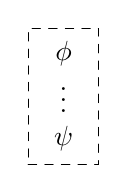
\begin{tikzpicture}
    \node [draw, rectangle, dashed, line cap=round]
    {\begin{tabular}{c} $\phi$ \\ \vdots \\ $\psi$ \end{tabular}};
  \end{tikzpicture}
  }{\phi \rightarrow \psi}
  \qquad \infer {
  \begin{tikzpicture}
    \node [draw, rectangle, dashed, line cap=round]
    {\begin{tabular}{c} $\phi$ \\ \vdots \\ $\bot$ \end{tabular}};
  \end{tikzpicture}
  }{\neg \phi}
  \qquad \infer {
  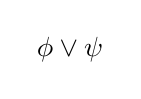
\begin{tikzpicture}
    \node {$\phi \lor \psi$};
  \end{tikzpicture} \\
  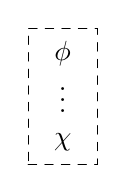
\begin{tikzpicture}
    \node [draw, rectangle, dashed, line cap=round]
    {\begin{tabular}{c} $\phi$ \\ \vdots \\ $\chi$ \end{tabular}};
  \end{tikzpicture} \\
  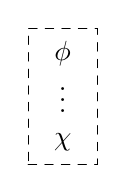
\begin{tikzpicture}
    \node [draw, rectangle, dashed, line cap=round]
    {\begin{tabular}{c} $\phi$ \\ \vdots \\ $\chi$ \end{tabular}};
  \end{tikzpicture}
  }{\chi}
\]

Using this notation, we can rewrite the proof for example
\ref{lecture_7:contrapositive}:
\[ \infer {
  \begin{tikzpicture}
    \node [draw, rectangle, dashed, line cap=round] {$
    \infer {
      \text{1. } \phi \rightarrow \psi \\\\
      \begin{tikzpicture}
        \node [draw, rectangle, dashed, line cap=round] {$
        \infer {
          \text{2. } \neg \psi \\\\
          \begin{tikzpicture}
            \node [draw, rectangle, dashed, line cap=round] {
            \begin{tabular}{c}
              3. $\phi$ \\
              4. $\psi$ ($\rightarrow$-elim, 1, 3) \\
              5. $\bot$ ($\neg$-elim, 2, 4)
            \end{tabular}
            };
          \end{tikzpicture}
        }{\neg \phi}
        $};
      \end{tikzpicture}
    }{\neg \psi \rightarrow \neg \phi}
    $};
  \end{tikzpicture}
  }{(\phi \rightarrow \psi)
    \rightarrow (\neg \psi \rightarrow \neg \phi)}
\]

The system defined above is in fact the NJ (Intuitionistic Natural 
Deduction) system. The NK system (Classical Natural Deduction) is NJ,
with the addition of the excluded-middle axiom:
\[ \infer* [right=ex-middle]
  { }{\Gamma \vdash \phi \lor \neg \phi}
\]

The NK system is sound and complete for propositional logic.

}} % End localization of command definitions
